%\documentclass[11pt, draft]{article}
\documentclass[11pt]{article}
\usepackage{lindrew}
\usepackage{xcolor}

\title{Physics 2301: Intermediate Mechanics II} \author{Lecturer: \textbf{Professor Anotonio Boveia}\\Notes by: Farhan Sadeek} \date{Spring 2025}

\begin{document}

\maketitle
%%%%%%%%%%%%%%%%%%%%%%%%%%%%
\section{January 7, 2025}
\subsection{Course Introduction}

Dr.\ Boveia talked about the course and we will head towards relativistic
mechanics. In this course we will master the concepts from Physics 1250 but
more broadly. \textbf{Tuesday} is the lecture day and \textbf{Wednesday,\space}
Thursday, and Friday are the problem-solving days. The grading scale would be
on \textbf{Standard Ohio State} grading scale. There might be a curve but it
will only curve up not down. Our grade would rely on \textbf{Quizzes (20\%),
Midterm (20\%), Final (20\%), Homework (30\%)}, and \textbf{Participation (10\%)}. The exams are \textbf{open-book, open-notes, and open-internet}.

\subsection{Success Tips}
Here are some tips to succeed in Physics 2301:
\begin{itemize}
    \item \textbf{Attend all lectures and problem-solving sessions:} Regular attendance will help you understand the material better and keep up with the course pace.
    \item \textbf{Stay organized:} Keep track of all assignments, quizzes, and exam dates. Use a planner or digital calendar to manage your time effectively.
    \item \textbf{Participate actively:} Engage in class discussions and ask questions whenever you have doubts. Participation counts towards your grade.
    \item \textbf{Form study groups:} Collaborate with your peers to discuss concepts and solve problems. Group study can provide different perspectives and enhance understanding.
    \item \textbf{Utilize office hours:} Take advantage of Dr.\ Boveia's office hours to seek clarification on topics you find challenging.
    \item \textbf{Practice regularly:} Consistently work on homework and additional problems to reinforce your understanding of relativistic mechanics.
    \item \textbf{Review notes:} Regularly review your lecture notes and summarize key points to aid retention.
    \item \textbf{Use available resources:} Make use of the textbook, online resources, and any supplementary materials provided by Dr.\ Boveia.
    \item \textbf{Stay healthy:} Ensure you get enough rest, eat well, and manage stress to maintain your overall well-being.
\end{itemize}
\subsection{Review of Vectors and Matrices}
\begin{definition}
    A \vocab{scalar quantity} is a quantity with numebrs for the most part.
\end{definition}

\begin{definition}
    A \vocab{vector quantity} is a triplet, with magnitude and direction. Vectors follow a different set of rules. For example, there are two multiplication rules for vectors: \textbf{Dot Product} and \textbf{Cross Product}. The dot product is a scalar quantity while the cross product is a vector quantity.

    \[
        |\vec{v}| = \text{Length and} \quad \vec{v} = \frac{|\vec{v}|}{\sqrt{3}}(V_x, V_y, V_z) \text{ if } \vec{v} = \langle V_x, V_y, V_z \rangle
    \]

    Scalar \(\times\) Vector = Vector \\ Vector \(\cdot\) Vector = Scalar (Dot
    Product or Inner Product) \\
    \[
        \vec{v} \cdot \vec{v} = V_x \cdot V_x + V_y \cdot V_y + V_z \cdot V_z = |\vec{v}|^2
    \]
    \[
        \vec{A} \cdot \vec{B} = A_x \cdot B_x + A_y \cdot B_y + A_z \cdot B_z = |\vec{A}| |\vec{B}| \cos \theta
    \]
    \[
        \vec{A} = A_x \hat{x} + A_y \hat{y} + A_z \hat{z} \]
    \(\hat{x}\) = `Unit Vector'
    \(|\hat{x}| = 1\)
    \[\vec{A} \cdot \vec{B} = (A_x \hat{x} + A_y \hat{y} + A_z \hat{z}) \cdot (B_x \hat{x} + B_y \hat{y} + B_z \hat{z}) = A_x B_x + A_y B_y + A_z B_z\]

    \(\hat{x}, \hat{y}, \hat{z}\) form an orthogonal normal basis, meaning that \(\hat{x} \cdot \hat{y} = 0\)
    \[\hat{x} \cdot \hat{y} = 0, \quad \hat{y} \cdot \hat{z} = 0, \quad \hat{z} \cdot \hat{x} = 0\]
    \[
        \hat{x} \cdot \hat{y} = 0, \quad \hat{y} \cdot \hat{z} = 0, \quad \hat{z} \cdot \hat{x} = 0
    \]
    Here, Ortho means that \(\hat{x} \cdot \hat{y} = 0\) and Normal means that
    \(\hat{x} \cdot \hat{x} = 1\)

\end{definition}

Vector \(\times\) Vector = Cross Product = Vector
\[
    \vec{A} \times \vec{B} = |\vec{A}| |\vec{B}| \sin \theta \hat{n}
\]

\[
    \vec{A} \times \vec{B} = \begin{vmatrix}
        \hat{x} & \hat{y} & \hat{z} \\
        A_x     & A_y     & A_z     \\
        B_x     & B_y     & B_z
    \end{vmatrix}
\]
\begin{tikzpicture}
    % Axes
    \draw[->] (0,0,0) -- (3,0,0) node[anchor=north east]{$x$};
    \draw[->] (0,0,0) -- (0,3,0) node[anchor=north west]{$y$};
    \draw[->] (0,0,0) -- (0,0,3) node[anchor=south]{$z$};

    % Vector A
    \draw[->, thick, blue] (0,0,0) -- (2,1,1) node[anchor=south west]{$\vec{A}$};

    % Vector B
    \draw[->, thick, red] (0,0,0) -- (1,2,1) node[anchor=south east]{$\vec{B}$};

    % Vector A x B
    \draw[->, thick, green] (0,0,0) -- (1,-1,3) node[anchor=north]{$\vec{A} \times \vec{B}$};
\end{tikzpicture}

\begin{figure}[h]
    \centering
    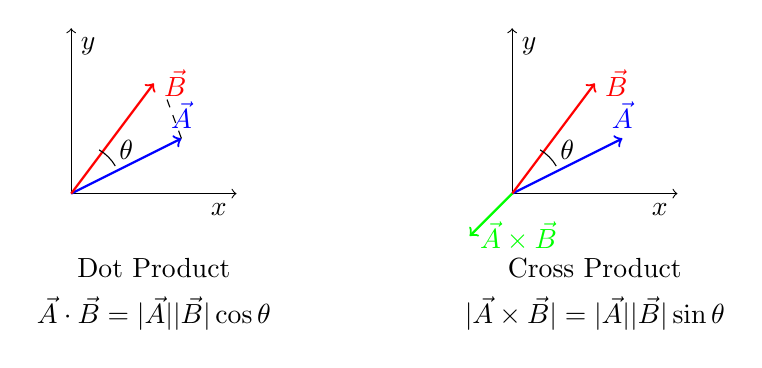
\begin{tikzpicture}[scale=0.7]
        % Axes for dot product
        \begin{scope}[xshift=-4cm]
            \draw[->] (0,0,0) -- (3,0,0) node[anchor=north east]{$x$};
            \draw[->] (0,0,0) -- (0,3,0) node[anchor=north west]{$y$};
            \draw[->, thick, blue] (0,0) -- (2,1) node[anchor=south]{$\vec{A}$};
            \draw[->, thick, red] (0,0) -- (1.5,2) node[anchor=west]{$\vec{B}$};
            \draw[dashed] (2,1) -- (1.73,1.73);
            \draw (0.8,0.5) arc (30:60:0.8);
            \node at (1,0.8) {$\theta$};
            \node[below] at (1.5,-1) {Dot Product};
            \node[below] at (1.5,-1.7) {$\vec{A}\cdot\vec{B} = |\vec{A}||\vec{B}|\cos\theta$};
        \end{scope}

        % Axes for cross product
        \begin{scope}[xshift=4cm]
            \draw[->] (0,0,0) -- (3,0,0) node[anchor=north east]{$x$};
            \draw[->] (0,0,0) -- (0,3,0) node[anchor=north west]{$y$};
            \draw[->, thick, blue] (0,0) -- (2,1) node[anchor=south]{$\vec{A}$};
            \draw[->, thick, red] (0,0) -- (1.5,2) node[anchor=west]{$\vec{B}$};
            \draw[->, thick, green] (0,0) -- (0,0,2) node[right]{$\vec{A}\times\vec{B}$};
            \draw (0.8,0.5) arc (30:60:0.8);
            \node at (1,0.8) {$\theta$};
            \node[below] at (1.5,-1) {Cross Product};
            \node[below] at (1.5,-1.7) {$|\vec{A}\times\vec{B}| = |\vec{A}||\vec{B}|\sin\theta$};
        \end{scope}
    \end{tikzpicture}
    \caption{Geometric interpretation of dot and cross products}
\end{figure}
\begin{tikzpicture}
    % Axes
    \draw[->] (0,0,0) -- (3,0,0) node[anchor=north east]{$x$};
    \draw[->] (0,0,0) -- (0,3,0) node[anchor=north west]{$y$};
    \draw[->] (0,0,0) -- (0,0,3) node[anchor=south]{$z$};

    % Vector A
    \draw[->, thick, blue] (0,0,0) -- (2,1,1) node[anchor=south west]{$\vec{A}$};

    % Vector B
    \draw[->, thick, red] (0,0,0) -- (1,2,1) node[anchor=south east]{$\vec{B}$};

    % Vector A x B
    \draw[->, thick, green] (0,0,0) -- (1,-1,3) node[anchor=north]{$\vec{A} \times \vec{B}$};
\end{tikzpicture}

\vocab{Dot product} is just the magnitude of the proejct of \(\vec{A}\) onto \(\vec{B}\).

$\vec{A} \times \vec{B} = |\vec{A}| |\vec{B}| \sin \theta \hat{n}$ [Magnitude] \\
Dot product is the component of $\vec{B}$ along $\vec{A}$. The dot product is a scalar quantity.

The cross product is a vector that is perpendicular to both \(\vec{A}\) and
\(\vec{B}\) (\(\vec{A} \perp \vec{B}\)). The magnitude of the cross product is
the area of the parallelogram formed by \(\vec{A}\) and \(\vec{B}\). The
direction of the cross product follows the right-hand rule.

    {The cross product is a vector that is perpendicular to both \(\vec{A}\) and \(\vec{B}\). The magnitude of the cross product is the area of the parallelogram formed by \(\vec{A}\) and \(\vec{B}\). The direction of the cross product follows the right-hand rule.}

\[
    \vec{A} \times \vec{B} = \begin{vmatrix}
        \hat{x} & \hat{y} & \hat{z} \\
        A_x     & A_y     & A_z     \\
        B_x     & B_y     & B_z
    \end{vmatrix}
\]
\section{January 8, 2025}

%\section{January 10, 2025}
%\section{January 13, 2025}
%\section{January 15, 2025}
%\section{January 17, 2025}
%\section{January 20, 2025}
%\section{January 22, 2025}
%\section{January 24, 2025}
%\section{January 27, 2025}
%\section{January 29, 2025}
%\section{January 31, 2025}
%\section{February 3, 2025}
%\section{February 5, 2025}
%\section{February 7, 2025}
%\section{February 10, 2025}
%\section{February 12, 2025}
%\section{February 14, 2025}
%\section{February 17, 2025}
%\section{February 19, 2025}
%\section{February 21, 2025}
%\section{February 24, 2025}
%\section{February 26, 2025}
%\section{February 28, 2025}
%\section{March 3, 2025}
%\section{March 5, 2025}
%\section{March 7, 2025}
%\section{March 17, 2025}
%\section{March 19, 2025}
%\section{March 21, 2025}
%\section{March 24, 2025}
%\section{March 26, 2025}
%\section{March 28, 2025}
%\section{March 31, 2025}
%\section{April 2, 2025}
%\section{April 4, 2025}
%\section{April 7, 2025}
%\section{April 9, 2025}
%\section{April 11, 2025}
%\section{April 14, 2025}
%\section{April 16, 2025}
%\section{April 18, 2025}
%\section{April 21, 2025}
%\section{April 23, 2025}
%\section{April 25, 2025}
%\section{April 28, 2025}

\end{document}